%  LaTeX support: latex@mdpi.com 
%  In case you need support, please attach all files that are necessary for compiling as well as the log file, and specify the details of your LaTeX setup (which operating system and LaTeX version / tools you are using).

%=================================================================
\documentclass[journal,article,submit,moreauthors,pdftex]{Definitions/mdpi} 

\usepackage{tabularx,colortbl}
\usepackage{booktabs} % For formal tables
\usepackage{array}
\usepackage{multirow}
\usepackage{subcaption}

\newcommand{\emad}[1]{\textcolor{red}{{\it [Emad: #1]}}}
\newcommand{\hosein}[1]{\textcolor{orange}{{\it [Hosein: #1]}}}
\newcommand{\todo}[1]{\colorbox{yellow}{\textbf{[#1]}}}

% If you would like to post an early version of this manuscript as a preprint, you may use preprint as the journal and change 'submit' to 'accept'. The document class line would be, e.g., \documentclass[preprints,article,accept,moreauthors,pdftex]{mdpi}. This is especially recommended for submission to arXiv, where line numbers should be removed before posting. For preprints.org, the editorial staff will make this change immediately prior to posting.

%--------------------
% Class Options:
%--------------------
%----------
% journal
%----------
% Choose between the following MDPI journals:
% acoustics, actuators, addictions, admsci, aerospace, agriculture, agriengineering, agronomy, algorithms, animals, antibiotics, antibodies, antioxidants, applsci, arts, asc, asi, atmosphere, atoms, axioms, batteries, bdcc, behavsci , beverages, bioengineering, biology, biomedicines, biomimetics, biomolecules, biosensors, brainsci , buildings, cancers, carbon , catalysts, cells, ceramics, challenges, chemengineering, chemistry, chemosensors, children, cleantechnol, climate, clockssleep, cmd, coatings, colloids, computation, computers, condensedmatter, cosmetics, cryptography, crystals, dairy, data, dentistry, designs , diagnostics, diseases, diversity, drones, econometrics, economies, education, electrochem, electronics, energies, entropy, environments, epigenomes, est, fermentation, fibers, fire, fishes, fluids, foods, forecasting, forests, fractalfract, futureinternet, futurephys, galaxies, games, gastrointestdisord, gels, genealogy, genes, geohazards, geosciences, geriatrics, hazardousmatters, healthcare, heritage, highthroughput, horticulturae, humanities, hydrology, ijerph, ijfs, ijgi, ijms, ijtpp, informatics, information, infrastructures, inorganics, insects, instruments, inventions, iot, j, jcdd, jcm, jcp, jcs, jdb, jfb, jfmk, jimaging, jintelligence, jlpea, jmmp, jmse, jnt, jof, joitmc, jpm, jrfm, jsan, land, languages, laws, life, literature, logistics, lubricants, machines, magnetochemistry, make, marinedrugs, materials, mathematics, mca, medicina, medicines, medsci, membranes, metabolites, metals, microarrays, micromachines, microorganisms, minerals, modelling, molbank, molecules, mps, mti, nanomaterials, ncrna, neonatalscreening, neuroglia, nitrogen, notspecified, nutrients, ohbm, particles, pathogens, pharmaceuticals, pharmaceutics, pharmacy, philosophies, photonics, physics, plants, plasma, polymers, polysaccharides, preprints , proceedings, processes, proteomes, psych, publications, quantumrep, quaternary, qubs, reactions, recycling, religions, remotesensing, reports, resources, risks, robotics, safety, sci, scipharm, sensors, separations, sexes, signals, sinusitis, smartcities, sna, societies, socsci, soilsystems, sports, standards, stats, surfaces, surgeries, sustainability, symmetry, systems, technologies, test, toxics, toxins, tropicalmed, universe, urbansci, vaccines, vehicles, vetsci, vibration, viruses, vision, water, wem, wevj

%---------
% article
%---------
% The default type of manuscript is "article", but can be replaced by: 
% abstract, addendum, article, benchmark, book, bookreview, briefreport, casereport, changes, comment, commentary, communication, conceptpaper, conferenceproceedings, correction, conferencereport, expressionofconcern, extendedabstract, meetingreport, creative, datadescriptor, discussion, editorial, essay, erratum, hypothesis, interestingimages, letter, meetingreport, newbookreceived, obituary, opinion, projectreport, reply, retraction, review, perspective, protocol, shortnote, supfile, technicalnote, viewpoint
% supfile = supplementary materials

%----------
% submit
%----------
% The class option "submit" will be changed to "accept" by the Editorial Office when the paper is accepted. This will only make changes to the frontpage (e.g., the logo of the journal will get visible), the headings, and the copyright information. Also, line numbering will be removed. Journal info and pagination for accepted papers will also be assigned by the Editorial Office.

%------------------
% moreauthors
%------------------
% If there is only one author the class option oneauthor should be used. Otherwise use the class option moreauthors.

%---------
% pdftex
%---------
% The option pdftex is for use with pdfLaTeX. If eps figures are used, remove the option pdftex and use LaTeX and dvi2pdf.

%=================================================================
\firstpage{1} 
\makeatletter 
\setcounter{page}{\@firstpage} 
\makeatother
\pubvolume{xx}
\issuenum{1}
\articlenumber{5}
\pubyear{2019}
\copyrightyear{2019}
%\externaleditor{Academic Editor: name}
\history{Received: date; Accepted: date; Published: date}
%\updates{yes} % If there is an update available, un-comment this line

%% MDPI internal command: uncomment if new journal that already uses continuous page numbers 
%\continuouspages{yes}

%------------------------------------------------------------------
% The following line should be uncommented if the LaTeX file is uploaded to arXiv.org
%\pdfoutput=1

%=================================================================
% Add packages and commands here. The following packages are loaded in our class file: fontenc, calc, indentfirst, fancyhdr, graphicx, lastpage, ifthen, lineno, float, amsmath, setspace, enumitem, mathpazo, booktabs, titlesec, etoolbox, amsthm, hyphenat, natbib, hyperref, footmisc, geometry, caption, url, mdframed, tabto, soul, multirow, microtype, tikz

%=================================================================
%% Please use the following mathematics environments: Theorem, Lemma, Corollary, Proposition, Characterization, Property, Problem, Example, ExamplesandDefinitions, Hypothesis, Remark, Definition
%% For proofs, please use the proof environment (the amsthm package is loaded by the MDPI class).

%=================================================================
% Full title of the paper (Capitalized)
\Title{Impact of Featureset on Cross-Trials and Cross-Subjects Evaluation for Human Activity Recognition }

% Author Orchid ID: enter ID or remove command
\newcommand{\orcidauthorA}{0000-0000-000-000X} % Add \orcidA{} behind the author's name
%\newcommand{\orcidauthorB}{0000-0000-000-000X} % Add \orcidB{} behind the author's name

% Authors, for the paper (add full first names)
\Author{Hosein Nourani $^{1,\dagger,\ddagger}$\orcidA{}, Emad Shihab $^{1,\ddagger}$ and Omid Sarbishei $^{2,}$*}

% Authors, for metadata in PDF
\AuthorNames{Hosein Nourani, Emad Shihab and Omid Sarbishei}

% Affiliations / Addresses (Add [1] after \address if there is only one affiliation.)
\address{%
$^{1}$ \quad Dept. of Computer Science and Software Engineering; h$.$nourani@hotmail.com\\
$^{2}$ \quad Dept. of Computer Science and Software Engineering; e$.$shihab@concordia.com}

% Contact information of the corresponding author
\corres{Correspondence: e-mail@e-mail.com; Tel.: (optional; include country code; if there are multiple corresponding authors, add author initials) +xx-xxxx-xxx-xxxx (F.L.)}

% Current address and/or shared authorship
\firstnote{Current address: Affiliation 3} 
\secondnote{These authors contributed equally to this work.}
% The commands \thirdnote{} till \eighthnote{} are available for further notes

%\simplesumm{} % Simple summary

%\conference{} % An extended version of a conference paper

% Abstract (Do not insert blank lines, i.e. \\) 
\abstract{Human Activity Recognition (HAR) refers to an emerging area of interest for medical, military, and security applications. However, the identification of the features to be used for activity classification and recognition is still an open point. In this work we have compared several state-of-the-art featuresets on HAR. To compare the featuresets, we have conducted an extensive set of experiments to indicate the vulnerable points in using featuresets. Aiming this goal, we implement several state-of-the-art machine learning models, ranging from traditional classifiers like SVM and GLM to convolutional neural networks; the models get evaluated by the performance gained using two challenging evaluation methods including cross-trials evaluation and cross-subjects evaluation, in addition to the convention method of 10-fold validation. The data from 55 gym exercises performing by thirteen subject have been recorded. To keep the realistic condition, they were asked to perform based on their own practice program. To capture the movements, two IMUs have been attached to the right wrist and right foot of the subjects. In total, 1300 features were extracted from the data. Our results showed that FNN acheived the highest performances using different featuresets. Against the prevailing wisdom, the statistical features gets outperformed by histogram feature set to deliver the best performance under all evaluation methods.
\hosein{After all, this work provides the intuitions behind 100 hand-crafted features for beginner and researcher in HAR }
	%(1) Background: Place the question addressed in a broad context and highlight the purpose of the study; (2) Methods: Describe briefly the main methods or treatments applied; (3) Results: Summarize the article's main findings; and (4) Conclusion: Indicate the main conclusions or interpretations. The abstract should be an objective representation of the article, it must not contain results which are not presented and substantiated in the main text and should not exaggerate the main conclusions.
}

% Keywords
\keyword{feature selection; featureset; Wearable; Motion sensor; Neural Network, Histogram, Human activity recognition }

% The fields PACS, MSC, and JEL may be left empty or commented out if not applicable
%\PACS{J0101}
%\MSC{}
%\JEL{}

%%%%%%%%%%%%%%%%%%%%%%%%%%%%%%%%%%%%%%%%%%
% Only for the journal Diversity
%\LSID{\url{http://}}

%%%%%%%%%%%%%%%%%%%%%%%%%%%%%%%%%%%%%%%%%%
% Only for the journal Applied Sciences:
%\featuredapplication{Authors are encouraged to provide a concise description of the specific application or a potential application of the work. This section is not mandatory.}
%%%%%%%%%%%%%%%%%%%%%%%%%%%%%%%%%%%%%%%%%%

%%%%%%%%%%%%%%%%%%%%%%%%%%%%%%%%%%%%%%%%%%
% Only for the journal Data:
%\dataset{DOI number or link to the deposited data set in cases where the data set is published or set to be published separately. If the data set is submitted and will be published as a supplement to this paper in the journal Data, this field will be filled by the editors of the journal. In this case, please make sure to submit the data set as a supplement when entering your manuscript into our manuscript editorial system.}

%\datasetlicense{license under which the data set is made available (CC0, CC-BY, CC-BY-SA, CC-BY-NC, etc.)}

%%%%%%%%%%%%%%%%%%%%%%%%%%%%%%%%%%%%%%%%%%
% Only for the journal Toxins
%\keycontribution{The breakthroughs or highlights of the manuscript. Authors can write one or two sentences to describe the most important part of the paper.}

%\setcounter{secnumdepth}{4}
%%%%%%%%%%%%%%%%%%%%%%%%%%%%%%%%%%%%%%%%%%
\begin{document}
%%%%%%%%%%%%%%%%%%%%%%%%%%%%%%%%%%%%%%%%%%

%%%%%%%%%%%%%%%%%%%%%%%%%%%%%%%%%%%%%%%%%%
%The order of the section titles is: Introduction, Materials and Methods, Results, Discussion, Conclusions for these journals: aerospace,algorithms,antibodies,antioxidants,atmosphere,axioms,biomedicines,carbon,crystals,designs,diagnostics,environments,fermentation,fluids,forests,fractalfract,informatics,information,inventions,jfmk,jrfm,lubricants,neonatalscreening,neuroglia,particles,pharmaceutics,polymers,processes,technologies,viruses,vision

\section{Introduction}

%The introduction should briefly place the study in a broad context and highlight why it is important. It should define the purpose of the work and its significance. The current state of the research field should be reviewed carefully and key publications cited. Please highlight controversial and diverging hypotheses when necessary. Finally, briefly mention the main aim of the work and highlight the principal conclusions. As far as possible, please keep the introduction comprehensible to scientists outside your particular field of research. Citing a journal paper \cite{ref-journal}. And now citing a book reference \cite{ref-book}. Please use the command \citep{ref-journal} for the following MDPI journals, which use author-date citation: Administrative Sciences, Arts, Econometrics, Economies, Genealogy, Humanities, IJFS, JRFM, Languages, Laws, Religions, Risks, Social Sciences.
%%%%%%%%%%%%%%%%%%%%%%%%%%%%%%%%%%%%%%%%%%
Human Activity Recognition (HAR) using inertial sensors has been a target of a lot of researches in the last decade. one reason is because it opens a door to the thousands of useful applications in healthcare, physical fitness monitoring, elder care support and etc. Another reason is due to the pervasiveness of wearable sensors. They are small in size, cheap, and already embedded in almost all wearable gadgets. This is a promising point for HAR applications since no extra hardware setup-cost is required for users to start using them immediately. This is to say that the most challenging part in HAR is to producing an application to be able to efficiently use the device's resources and deliver the most accurate result in the form of classifying the activity type or counting it \cite{schilit1994context}.\\
Basically, a HAR system using Inertial Measurement Units (IMUs) is composed of two basic components: (1) a data acquisition unit responsible for capturing human movements, (2) a processing unit responsible for recognizing the certain activities among movements of the subject\cite{rosati2018comparison}. In the first component, the human movements is captured by different motion sensors such as accelerometer, gyroscope, and so on. These sensors can be located in an off-the-shelf device like a smart-phone for general HAR applications or specifically are accompanied by a storage and a processor, formed a System on Chip (SoC) for a certain purpose.\\
The captured movements as raw data transmits to the second component for processing operation. Within this component, there is a pattern recognition (HAR) model that classifies the input signals into certain classes of activities. This HAR model typically consists of three phases. First, there is a pre-processing operation that extracts informative features from raw signal. Second, a classifier is trained over extracted features. Third, an evaluation method to ensure that the classifier provides the required performance\cite{kolodziej2019registration}. In other words, a HAR model should address these three aspects to be able to recognize an activity. The previous studies have achieved many improvements in each stages[][][] however there are challenging aspects that they did not contemplate them and they are still open:
\begin{itemize}[leftmargin=*,labelsep=5.8mm]
	\item	Identifying the correct set of input features for the classifier\cite{rosati2018comparison} (in the phase 1)
	\item	Existing an unique and reliable validation protocol to assess the models \cite{jordao2018human}(in the phase 3)
\end{itemize} 
%(3) impact of quality of dataset on performance since they vary from paper to paper\cite{jordao2018human}.\\
%While the first two issues have impact on performance of a model in general, the third one influences directly on recognition result, independent from how much a model is well designed. Factors like size of dataset, frequency rate of sensors, complexity of target activities, sensor position and how it is attached to the body, and so on. In [], the authors, looking for impact of sensor alignments, in two different trials attached the sensor to the subjects. In first trial, an expert attached the sensor while in the second trial, subjects were asked to attached the sensors by themselves. Results show that the performance has a significant collapse during the second trials.
%
While the first issue plays an important role to improve the performance of the model, the second issue is a critical point since different validation methods show the performance differently, somehow biased. For the same reason, using HAR models on new dataset shows a significant decrease in performance. As a consequence of this issue, currently it is impossible to know the state-of-the-art methods in human activity recognition\cite{jordao2018human}. Addition to this, some factors like temporal changes in user body (e.g., tiredness) have impacts on how they perform an identical activity within two different trials. However, it is impossible to evaluate such impacts by using the the traditional validation methods like k-fold cross-validation or Leave-One-Subject-Out (LOSO). To address this issue, in this study, we employ Leave-One-Trial-Out (LOTO) cross-validation addition to conventional validation methods. Using this validation method, we show that how the performance and robustness of the model change by feeding it by more trials.\\
Regarding the first issue, previous works have employed a wide range of features for HAR model. Dealing with selecting appropriate features for a HAR model (feature selection methods) are usually aiming to improve the performance of the model. However in \cite{rosati2018comparison} which is the most similar previous work to us, the authors also listed three extra issues which less have been considered in previous works:
(1) The processing cost of producing a feature
(2) The complexity of calculation of features makes a model difficult to understand.
(3) The negative impacts of having too much number of features on performance of the model.
In our previous work\cite{Nourani_CoMoRea2019}, we showed that by removing redundant features, we can keep the performance identical while shrink the dataset to 8\% of its initial size. This approach significantly decreases the processing cost and vulnerability of getting overfit. In this study, we will focus on decreasing \textbf{the complexity of calculation of features} rather just decreasing size of dataset in a feature-set.\\

The aforementioned discussion motivated our study, where we evaluate a wide range of features by the performance reached by six popular classifiers. The models train and evaluate on two huge datasets (include our dataset which is one of the biggest dataset on gym exercises, publicly available). To provide a more robust evaluation we validate our models under several cross-validation methods.

The aim of this article is to present the following main contributions:
\begin{itemize}
	\item Implementation and evaluation of the remarkable state-of-the-art featuresets.
	\item Analysing the impact of temporal changes on HAR model.
	\item Proposition of a novel model using Forward Neural Network (FNN) in HAR
\end{itemize}
Regarding the target datasets, we chose [] dataset since it provides a wide range of activities (33 activities) and it is big enough. However, to the best of our knowledge, there is no dataset that targets different trials of same activity with same subject, publicly available. So, we collected a dataset of 15 subjects and +50 gym activities including different trials for each activity.

The rest of this paper is organized as follows. Section 2 describes the study setup including the approach and the dataset used in this study. Section 3 defines the featuresets and theirs advantages in previous works. Section 4 presents the results of using featuresets on classifiers. Finally, Section 7 summarizes this study and highlight the most important contributions of this paper for future works.
\section{Related Work}
To the best of our knowledge, the statistical functions on time-domain signal provide the most popular features in HAR. Features like mean, median, mean standard deviation, variance, minimum, maximum are the most popular ones. The second group, Frequency-domain features are so helpful for those models that target periodic activities like walking. To achieve a frequency-domain feature, one segment of time signal should be transferred to several components in frequency domain. Each component may/may not have meaning depend on the activity. Frequency bins and auto-correlation coefficient are some example.

Suto et al., 2017 investigate the efficiency of the popular machine learning strategies based on a right-ankle-mounted accelerometer, and their results suggest that one sensor is not enough for appropriate daily activity recognition due to the similar data generated from one sensor for different activities
Generally, One to One is the basic deployment and more suitable for the basic recognition tasks, such as step counting or sleep quality monitoring
Placing more sensors on multiple body parts is intuitively beneficial for improving the performance and robustness, whereas this can also result in increased complexity in deployment and computation cost
Sztyler et al., 2017 develop a position-aware HAR system by placing seven accelerometers in different body positions
\section{Data}

The most crucial requirement to start an activity recognition process is having the real-world data of human activities. Although there are couple of datasets publicly available for HAR\cite{wang2019survey}, to the best of our knowledge, non of them provide the data of different sessions (neither at same day or different days) of same subject. In addition, they mostly focused on daily routine activities rather transition activities (e.g., gym exercises) which are repetitive and more complicated in terms of pattern recognition\cite{wang2019survey}. Therefore, in this study we collect a dataset providing the following features:
\begin{itemize}[leftmargin=*,labelsep=5.8mm]
	\item Specifically targeted on regular gym activities (including 55 exercises)
	\item The data tracks activities of a set of subjects over two to six weeks
	\item Data is recorded by four sensors (two wrists and two foots)
	\item Subjects performed the practices only based on their own experiences (there is no instruction) 
\end{itemize}
To aim this goal, the first step is to determine the sensor type and how to deploy a system to collect the data. In this work, we have employed a SoC device which called \textit{Neblina}.
\subsubsection{Neblina}
Neblina is a miniature-sized box containing three tri-axial motion sensors (accelerometer, gyroscope, magnetometer) along with a processor, a flash memory, battery, and a bluetooth port. Using blue-tooth port, it can transmit the result to a host (e.g., cellphone or desktop computer).  In fact, Neblina is equipped with all requirements for a real-time HAR system. Comparing with a smartphone, Neblina is much smaller (Figure \ref{neblina_setup}) that lets us to attach it to different part of the subject's body without making any interrupt in his/her actions\cite{de2018comparative}. Having access directly to different resources like sensors or memory without OS interferences is another advantage of using Neblina that let us improve the efficiency of the model.
\begin{figure}[H]
	\centering
	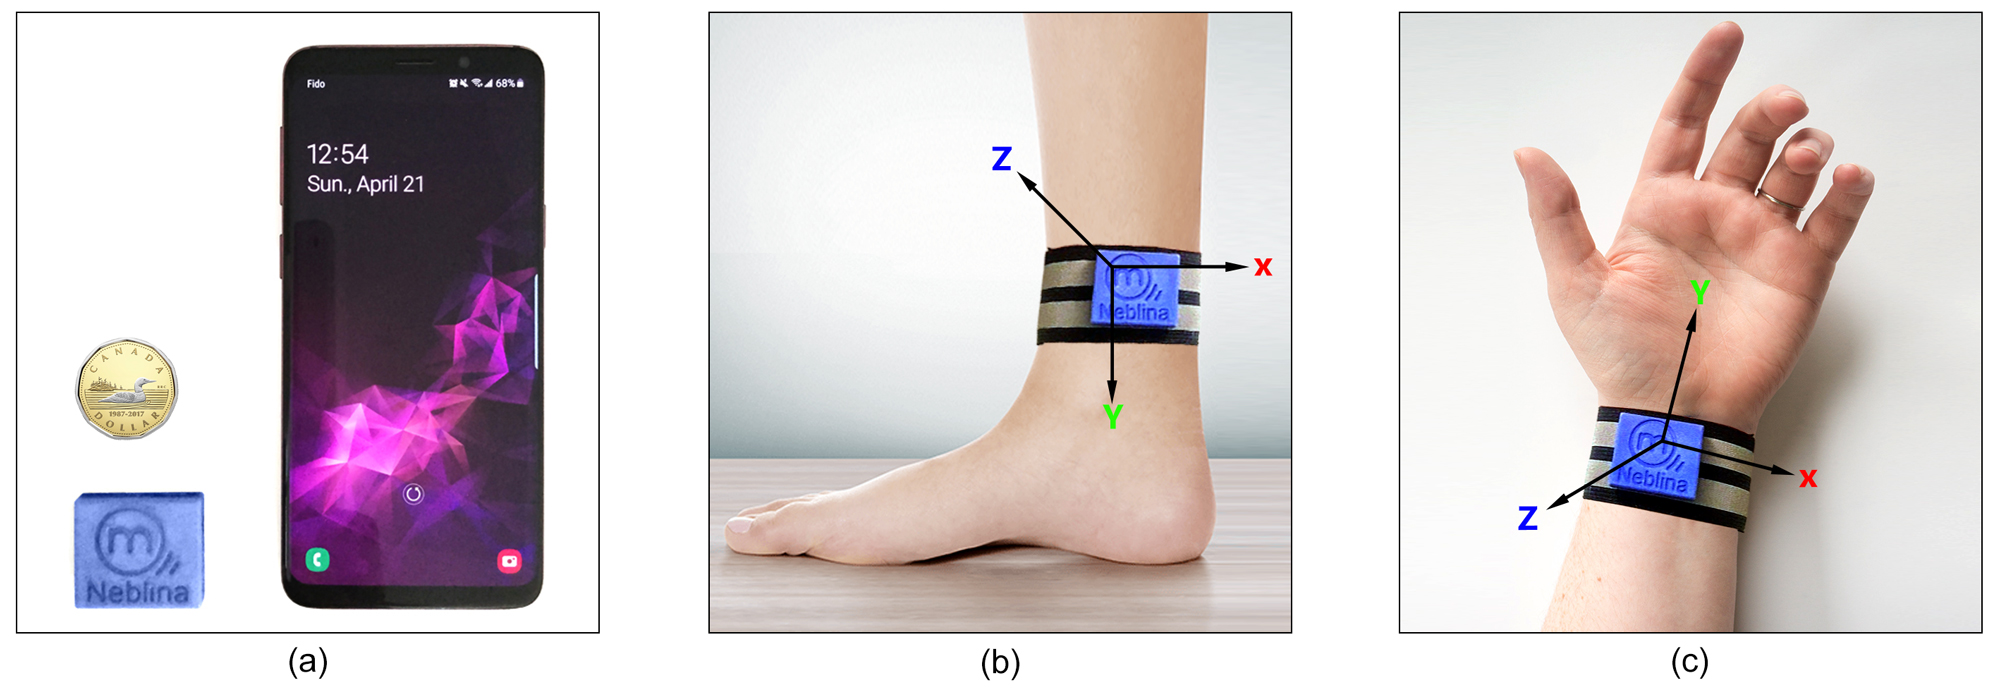
\includegraphics[width=10 cm]{Definitions/images/neblina_setup.jpg}
	\caption{Neblina setup. (a) Compares dimensions of Neblina with a 1 dollar coin and a cellphone (Sumsung Galaxy s9). (b) How Neblina located on foot using a strap. (c) How Neblina located on wrist using a strap.}
	\label{neblina_setup}
\end{figure} 
\subsubsection{Sensors} 
Depending on how much an activity is complicated (e.g., how many part of body are involved or how many stages are involved in it), a researcher may need to attach one or more sensors on different positions of the human body. However, using more sensors affects usability negatively. From the literature, using sensor on wrist for most of upper activities and using a sensor on foot for lower-body activity are more effective than other locations including chest, waist, thigh and so on. In this study, to cover activities both on lower-body and upper-body, two sensors were attached to right wrist and right foot (Figure \ref{neblina_setup} (b) and (c)). Although the device provides the magnetometer signals, we limited our process on using the accelerometer and gyroscope signals only. It is because the magnetometer signal can be affected by getting close to iron equipments in the gym. The frequency rate is fixed on 50Hz. It is worth to mention that the frequency rate more than 50Hz is not necessary because according to the Nyquist theorem, this rate is enough to record a repetitive activity with 25 cycle per second which is so much faster than the iterations of normal workouts in the gym (one iteration per 1-5 seconds).\\
\subsection{Subjects}
We asked 15 members of a gym (4 female), ages 21-35, to participate in this study. Participants varied in level of expertise (from 1 month to 6 consecutive years of experience). For more realistic scenarios, we did not constrain participants to certain exercises, instead we asked them to follow up their own plan. Comparing with previous works' dataset, considering this level of freedom for subjects returns following advantages: (1) Since each session is about 1 to 2 hours, we can observe the impact of fatigue on performing an activity. (2) The unknown period or null-class activities are not artificially performed, since subjects were free to do whatever they normally do in gym (3) impact of background experience can be measured. It is because the gym programs are cyclic over week or month. By repeating an activity over cycles, Subjects will be more consistent over different sets ( a consecutive sequence of doing one activity). (4) there is no instruction of how doing exercises for subjects. Although this can let subjects to perform an activity in non-identical way, it is considered as an advantage for our study since it replicates the real-world condition. In \cite{morris2014recofit}, the authors showed that by changing the environment from space-constrained laboratory to a real gym the segmentation performance for recognizing gym exercises has dropped by 50\%. Therefore, another advantage of keeping the experiment under real-world condition is the performance of the model is more reliable.\\
\subsection{Activities}
Our dataset ended up with 55 common exercises in gym. During electing participants, we picked mostly those persons who do more common exercises involved in either upper body or lower body. Thus, activities like Wall ball, jumping jacks and so on or advanced exercise in body-building are not in our dataset. In \cite{soro2019recognition} (the second dataset in this work), authors have targeted CrossFit activities which are involved in upper and lower body together. They have shown that only one sensor on wrist is enough to recognize such activities. Therefore, in this study we focused on those exercises in which either lower or upper body keeps stable during the activity. Thereby, existing the second sensor is necessary for recognizing the activity. As listed in Table \ref{activity_list}, only two activities are involved in both upper and lower body. Running on treadmill (A1) make lower body involved. While In previous works this activity was recognized by sensor on wrist. Since a user can put her/his hands on device handler, using sensor on wrist is not effective always. \\
\hosein{Recognition accuracy is assessed in the context of a circuit, and inevitably the choice of circuit affects accuracy. A larger number of activities or high similarity among activities will reduce accuracy. Comprehensive analysis of all possible circuits is prohibitive, so we present results from the two circuits used in our study, along with leave-one-out cross-validation results from our training data for two reasonable circuits of different sizes, to demonstrate the effect of circuit size on accuracy.}
\begin{table}[H]
	\caption{List of exercises along with target body part involved in each exercise.}
	\centering
	%% \tablesize{} %% You can specify the fontsize here, e.g., \tablesize{\footnotesize}. If commented out \small will be used.
	\begin{tabular}{ccc}
		\toprule
		\textbf{Exercise}	& \textbf{Body Involved}	& \textbf{Code}\\
		\midrule
		Lat Pull Down		& upper 		& A1\\
		Bench Press		& upper 			& A2\\
		Biceps curl		& upper			& A3\\
		Push-ups & upper			& A4\\
		Treadmill		& lower 			& A5\\
		Ab crunch machine		& lower \& upper & A6\\
		Reverse Crunch & lower			& A7 \\
		Russian Twist & lower			& A8 \\
		\bottomrule
	\end{tabular}
\label{activity_list}
\end{table}
\subsection{Data points}
To generate the data points, previous works have employed different strategies. One well-known method for time-series signals is sliding-windows. As long as an activity is squashed in a range of samples during time, a model can see a stream of recorded data through a window with limited length of seconds (e.g., in this study it is 5 seconds time window). This window slides through the stream with a certain step size called shifting size. As long as the shifting size smaller than widow size, the sliding window is called overlapping and non-overlapping if they are equal. Previous works have shown that the different lengths of window size and shifting size influence the performance of the model and the computational cost. Because the activities in this study are gym exercise which the do not take longer than 5 seconds, intuitively, we choose 5 seconds for window size. It is a safe window size to ensure that at least one cycle of the activity can be completely seen in a window frame. we defined 200 milliseconds for shifting step which keeps the model more sensitive against changes in signal at the expense of more computational cost. Having such small shifting step does make sense since in real-world applications it decreases the latency of the application on predicting the activity type. Addition to the time period, the window length can be defined by the sampling rate of sensor. In this work, the sample rate is 50Hz. So, each window contains 250 (5 * 50) samples.

\subsection{Dataset}
To label the data we employed a process including three phases: (1) Before beginning of each session, each subject was asked to fill a form about list of activities, number of sets, and the weights if applicable. (2) During the session, a supervisor manually records type of exercise, the moment of start and stop, and number of repetitions. (3) After finishing the session, in order to have our desired accuracy in labelling, we visually trace the signals of accelerometer and gyroscope to refine the regains assigned to each exercise.
Table \ref{dataset_statistics} shows the statistics of the dataset. Since subjects may participate in more than one session, next column after subjects, shows the total number of sessions for each activity.  , in the initial dataset, the number of subjects who are involved in all exercises is not equally distributed. Although  Thus, we defined four datasets corresponding with our four experiments including K-fold evaluation, Leave-One-Set-Out evaluation, Leave-One-Session-Out evaluation, and Leave-One-Subject-Out evaluation.
\begin{table}[H]
	\caption{Statistics of the dataset divided by type of exercise along with the experiments that involve them in.}
	\centering
	%% \tablesize{} %% You can specify the fontsize here, e.g., \tablesize{\footnotesize}. If commented out \small will be used.
	\begin{tabular}{cccccccc}
		\toprule
		\textbf{Exercise} & \textbf{Subjects} & \textbf{Sessions}	 & \textbf{Reps} & \textbf{Samples} & \textbf{10-fold} & \textbf{LOSO} & \textbf{LOTO} \\
		\midrule		
		Lat Pull Down& 6& 22& 218& 14700& Yes& Yes& Yes\\
		Bench Press	& 6& 26& 273& 23230& Yes& Yes& Yes\\
		Biceps curl	& 4& 13& 115& 16095&Yes& Yes& No\\
		Push-ups & 5& 16& 181& 9200& Yes& Yes& Yes\\
		Treadmill& 4& 5& +1200 & 68780& Yes& Yes& Yes\\
		Ab crunch machine& 3& 12& 108 & 10580& Yes& No& Yes\\
		Crunch Twist &  3& 12& 98& 8760& Yes& No& Yes\\
		Russian Twist & 3& 8& 67& 8520& Yes& No& Yes\\
		\bottomrule
	\end{tabular}
	\label{dataset_statistics}
\end{table}
\section{Method}
A typical work-flow on human activity recognition is including pre-processing, feature extraction, classification and evaluation. The process is shown in Figure \ref{???}. In this work we investigate the impact of 5 different featuresets in feature extraction phase; 5 different classifiers on classification phase; and 3 validation methods in evaluation phase.
\subsection{Pre-processing}
In this work, the common pre-processing operation for all experiments is a scale normalization. In fact, we scale all the input signals into a range between 0 and 1. Nevertheless, in some cases based on the requirements of the featuresets we add an extra layer of pre-processing which will be explained in related section.
\subsection{Feature Extraction}
In literature, in order to gain more information from the sensory data, the authors came up with hundreds of hand-crafted features among time domains, frequency domain or a combination of them. While each feature represents the signal in a certain point of view, it does not mean that this feature is informative enough for a model to recognize an activity based on that. One decisive factor to build a new feature is respecting the type of activity. Wang et. al. in \cite{wang2019survey} categorized human activities based on velocity and complexity (number of phases) of an activity into three main groups: (1) The \textbf{basic activities} which happen in comparatively longer duration e.g., walking and running. (2)  The complex activities that are in the form of a sequence of several phases. Each phase might be a complex or basic activity e.g., coffee time, smoking. (3) Transition activities which having a certain but temporal pattern happening between two different postures or two basic activities. e.g., stand-to-sit, push-ups and so on. From this point of view, previous works introduced  different feature sets that each one target a given type of activity. Consequently, targeting more than one type of activity brings more challenges for researcher to create a suitable set of features. Since exercises in gym composed of an orchestration of different type activities (basic, transition, complex), presenting a model to effectively recognize these activities will be more challenging. In this work, we compare the most state-of-the-arts feature sets in the literature. It is important to mention that we selected the ones that provide enough information to reproducibility (e.g., the definition of the features).
\begin{table}[H]
	\caption{Statical Functions along with the definitions and abbreviations }
	\centering
	%% \tablesize{} %% You can specify the fontsize here, e.g., \tablesize{\footnotesize}. If commented out \small will be used.
	\begin{tabular}{p{0.9cm}p{5cm}p{7cm}p{1.3cm}}
		\toprule
		\textbf{Code} & \textbf{Function} & \textbf{Description/Intuition} & \textbf{{\scriptsize abbreviation}} \\
		\midrule
		{\footnotesize S1}&Minimum & {\scriptsize The value of the least sample}& MIN\\
		S2&Maximum & {\scriptsize The value of the greatest sample}& MAX\\
		{\footnotesize S3, SS8}&Mean&  {\scriptsize The average of all samples}& MEA\\
		{\footnotesize S4}&Median&  {\scriptsize The middle value of samples}& MEA\\
		{\footnotesize S5}&{\footnotesize Mean Absolute Deviation}& {\scriptsize The average distance between each sample and the mean of the stream}& MAD\\
		{\footnotesize S6}&{\footnotesize Median Absolute Deviation}& {\scriptsize The average distance between each sample and the median of the stream}& MAA\\
		{\footnotesize S7}&Inner Quartile Range  & {\scriptsize The amount of spread in the middle part \%50 of the stream}& IQR\\
		{\footnotesize S8}&Mean Crossing Rate& {\scriptsize The rate of passing the mean along the stream}& MCR\\
		{\footnotesize S9, SS9}&Standard Deviation& {\scriptsize how far the samples are from the mean}& SD\\
		{\footnotesize S10, SS10}&Variance& {\scriptsize the average degree of distance between samples and mean}& VAR\\
		{\footnotesize S11, SS11}&Root Mean Square& {\scriptsize The square root of the arithmetic mean of the squares of samples}& RMS\\
		{\footnotesize HB}& Histogram Bin&{\scriptsize a 20 bins distribution of data } & Hbin (1-20) \\
		{\footnotesize SS1}&Number of autocorrelation peaks& {\scriptsize The greater number of peaks refers to non-periodic activity and vice versa. }& NAcP\\
		{\footnotesize SS2}&Prominent autocorrelation peaks&{\scriptsize NAcP with an extra condition that the peaks should be greater than neighbours with at least a certain distance} & NAcPP \\
		{\footnotesize SS3}&Weak autocorrelation peaks&{\scriptsize NAcP with an extra condition that the distance between the peaks and neighbours should be less than a certain distance} & NAcWP \\
		{\footnotesize SS4}&Maximum autocorrelation value&{\scriptsize Value of the greatest peak (except for the initial peak at zero lag)} & MAXAc \\
		{\footnotesize SS5}&Height of the first autocorrelation peak (after zero-crossing)&{\scriptsize less height refers to more fluctuations within the stream  } & FAcP \\
		{\footnotesize SS6}&Power bins (10 bins)&{\scriptsize A 10 bins distribution of amplitudes of frequencies from 0.2-25Hz    } & Pbin(1-10) \\
		{\footnotesize SS7}&Integrated RMS&{\scriptsize The root-mean-square amplitude of the signal after cumulative summation } & IRMS \\
		Ph1&Movement Intensity&{\scriptsize the Euclidean norm of the total acceleration vector after removing the static gravitational acceleration } & MI\\
		Ph2&Normalized Signal Magnitude Area&{\scriptsize the acceleration magnitude summed over three axes within each window normalized by the window length } & SMA \\
		Ph3&Eigenvalues of Dominant Directions&{\scriptsize The eigenvectors of the covariance matrix of the acceleration data correspond to the dominant directions along which intensive human motion occurs.} & \\
		Ph4&Correlation between Acceleration along Gravity and Heading Directions&{\scriptsize It shows the human movement is either vertically or horizontally. } &CAGH \\
		Ph5&Averaged Velocity along Heading Direction&{\scriptsize The Euclidean norm of the averaged velocities along y and z axes over the window.} &AVH \\
		Ph6&Averaged Velocity along Gravity Direction&{\scriptsize averaging the instantaneous velocity along the gravity direction at each time t over the window } & AVG \\
		Ph7&Averaged Rotation Angles related to Gravity Direction&{\scriptsize The cumulative rotation angles around gravity direction} & ARATG \\
		Ph8&Dominant Frequency&{\scriptsize The frequency corresponding to the maximum of the squared discrete FFT component magnitudes of the signal from each sensor axis} & DF \\
		Ph9&Energy&{\scriptsize The sum of the squared discrete FFT component magnitudes of the signal from each sensor axis} & ENERGY \\
		Ph10&Averaged Acceleration Energy&{\scriptsize The mean value of the energy over three acceleration axes} & AAE \\
		Ph11&Averaged Rotation Energy&{\scriptsize The mean value of the energy over three gyroscope axes. } & ARE \\
		OI1&Orientation Independent&{\scriptsize result of applying PCA on Single Value Decomposition  of x/y/x values of the stream } & PCASVD(1-30) \\
		%		&&{\scriptsize } & \\
		%		&&{\scriptsize } & \\
		%		&&{\scriptsize } & \\
		\bottomrule
	\end{tabular}
	\label{features_table}
\end{table}
\subsubsection{Set\_A: Statistical Features (ST\_Set)}
Time-domain features are those features obtained directly from a window of sensor data and are typically statistical measures. They have been intensively investigated in different applications and proved to be effective and useful for HAR. These features are based on a comprehensive and intuitive understanding of how a specific activity or posture will produce a set of discriminative features from measured sensor signals. Lots of studies used statistical features in their work because of the reasons mentioned above as well as the low computational cost of them. Set A composed of 20 features based on applying 10 statistical functions on 12 input time-domain signal including (x/y/z axes of accelerometer and gyroscope, along with the cumulative sums of those axes). Table \ref{features_table} shows the functions and a short description about each of them.


\subsubsection{Set\_B: Histogram bins Features (HB\_Set)}
The histogram representation of a time series signal is equal to the probability distribution of that signal over a period of time (window size). In HAR, considering the fact that each activity contains a set of small movements (as small as one sample) with certain acceleration and rotation, histogram can indicate the difference between activities by showing the different distributions of those small movements. Comparing with other statistical features, extracting histogram bins is low cost in terms of required processing time and memory usage\cite{Sarbishei2019platform}. In this work we consider 20 bins to distribute the data among them (HB in Table \ref{features_table})

\subsubsection{Set\_C: Self-Similar Features (SS\_Set)}
Although by having enough number of bins, histogram can show the trend of data, they can not display the individual times, nor the iterations within the data. In addition, an exercise activity is inherently repetitive rather than a non-exercise activity. In other word, the signal from non-exercise activities looks more stochastic in a short period of time. Set C is designed based on the idea of extracting repetitions from the signal. This attribute of human activity can be extracted by calculating the convolution of a signal with shifted version of itself (autocorrelation) as well as by extracting the components of signal at frequency domain. Authors in \cite{morris2014recofit} leveraged both methods (the autocorrelation and frequency functions) to make a featureset (self-similar features) to recognize gym exercises. This feature-set contains 160 features. They prepared 8 input signals including: 
\begin{itemize}
	\item The x axis of each sensor\\
	\item The magnitude of the accelerometer and gyroscope. \\
	\item The first principal component of all axes of each sensor.\\
	\item The first principal component of y and z axes of each sensors.\\
\end{itemize}
Table \ref{features_table} shows the list of all features that are employed in this feature set (SS1-SS11) along with the intuition behind each of them.
%\hosein{from implementation point of view: in their experiments: the X axis of the sensor corresponds to the vector along the user’s arm however in our case y axis is toward arm's direction}
\subsubsection{Set\_D: Physical Features (PH\_Set)}
One idea to design more informative features from sensory data is to bring the principles of human movements into consideration. Specifically this type of features are derived based on the physical interpretations of human motion which called physical features. In \cite{zhang2011feature}, the authors introduced a set of features based on physical parameters of human motion. To have an strong physical meaning of motion data (e.g., moving forward, backward), they assumed that the sensor position and direction are known during the experiment. Comparing with previous featuresets, these features made up from a fusion of multiple inputs rather just applying a function on one input. As a part of pre-processing operation for some of their features, they mentioned that they remove gravity from acceleration but they did not reveal any formula for that. In this paper, we remove the gravity using gyroscope data by applying the method described in \cite{Accelero5:online}.
%\hosein{Although this assumption limits the generalization of our physical features to be applied to other locations and orientations to some extent, it simplifies the problem and allows us to focus on designing features with strong physical meanings so as to better describe human motion1.}
%
%\hosein{regarding feature movement Intensity, the author did not mention that how they remove gravity from acceleration. I found a formula that uses gyroscope information to remove gravity. However this method can not be very accurate since at some situations like freely dropping, the linear acceleration is zero while the formula says something rather zero. generally speaking, it is not very accurate for detecting shake (fast movements) }
%Similar to set B, in this feature-set the sensor fusion is performed at pre-processing level.

\subsubsection{Set\_E: Orientation Independent Features (OI\_Set)}
In contrast to physical features which is dependant to the position and orientation of the sensors, in \cite{yurtman2017activity}, Yurtman et. al. targeted on a HAR model that does not rely on the variation of sensor orientation. In fact, in their model, they introduced an Orientation-invariant transformations (OITs). They compared their model with the ordinary model - pre-defined sensor orientation, on five different datasets. Although their featureset did not have a significant impact on performance, it brought an extra added value to the model that lets the model to be more robust against orientation. The OIT that they have introduced in their work is inspired by the idea of \textit{single value decomposition}\cite{moon2000mathematical}. First, they project every data point from original x/y/z space to a new space with same number of dimensions but with largest distance between data points. The intuition here is that the direction of the axes are defined by value of the data points not by x, y or z direction. Next, they apply PCA on transformed data and take first 30 most informative features. In Table\ref{features_table}, these type of features  are indicated by "OI" prefix.

%\subsection{Feature Selection}
%\hosein{we may not want to delete this section}
%However, using all extracted features to train a model does not guarantee the model to deliver best performance in recognition. There are two major objectives in feature selection phase that need to be achieved: 
%a.	finding a set of minimum redundant features
%b.	finding a set of maximum relevant features
%Feature selection methods have also other responsibilities like preventing model from being over fitted, suffering from curse of dimensionality, and delivering a visual presentation of the feature space to data analyst to let him/her to figure out the level of complexity of the project in hand. 

\subsection{Activity Recognition}
\hosein{high-level Description => Based on Activity Recognition Chain (ARC) in \cite{bulling2014tutorial}}
\hosein{Comparing the process between classical models VS Neural Network model}

In the well-known paper \cite{bulling2014tutorial}, the authors have described the main characteristics of a HAR model into five categories. They categorized the HAR models by: (1) execution type (offline/ online), (2) type of the activities that the model can recognize (Periodic/Sporadic/Static), (3) type of input signal (segmented/ continuous) (4) dependency of model to the user (user-independent/ user-specific), (5) dependency of model to the other inputs like user's context (stateless/ stateful).  In this study, models are \underline{stateless} and work on \underline{segmented stream} in \underline{offline mode}. Regarding dependency of model to the user, in this study, we investigate different aspects of user that can influence the performance of the model.\\

\subsubsection{Support Vector Machine}
Assuming each data point is a co-ordinate (support vector) of feature space, the Support Vector Machine (SVM) is an algorithm to find an optimum hyperplane between support vectors between two classes. To create a more robust classification, SVM maximises the distance between the hyperplane and the closest support vectors of each class (margin); This happens at the expense of increasing the tolerance(mis-classification) of the model (loss function). In a situation that finding a hyperplane between two classes is impossible, the SVM project the feature space to another space having more number of dimensions. This is the responsibility of a function called Kernel function.
\subsubsection{Decision Tree}
Assuming a training set size of N samples and M features, an ensemble of K decision trees (weak learners) is called RF such that in the training phase, each tree in the classifier randomly picks a set of training samples (n<<N) via bootstrapping and it finds the best split from a set of randomly selected features (m<<M). To get the class labels in the test phase, the class probabilities at leaf nodes of the trees are averaged and the highest average probability is chosen as the class label of the input sample.

\subsubsection{K-nearest neighbour}
KNN algorithm is a simple classification algorithm based on the calculation of the distance
(usually the Euclidean distance) between the new element to be classified and the elements in the training set. Firstly, the training elements are sorted in descending order according to their distance from the new element. Then, the most frequent class of the first K elements (called neighbors) is associated to the new element. For this kind of classifier, only the value of the K neighbors must be decided. A common starting N, where N was the number of elements in the training set. Beginning from
value for K is $ K_{in} $
this consideration, we decided to analyze 32 values around Kin and, thus, we used five bits for the second substring of each GA solution (25 = 32): each possible value assumed by the second substring was associated to a specific K value to be set in the classifier.
\subsubsection{Forward Neural Network}
A FNN is made up of a set of neurons, connected by weighted arcs, that process the input
information according to the McCulloch and Pitts model:
\begin{equation}\label{fnn_formula}
 y = f(\sum_{i}^{}w_{i}.x_{i})
\end{equation}
where y is the output of the neuron, wi are weights of the incoming connections, xi are inputs to the neuron, and f is called transfer function and should be selected according to the classification problem.\\
Neurons in a FNN are organized in layers: in the input layer, one neuron for each input variable is required; the number of neurons in the output layer is decided according to the number of classes to be recognized and the selected transfer function; between input and output layers a certain number of hidden layers can be inserted, whose dimensions are usually decided testing different configurations. \\
An ANN consists of neurons, each of which produces an output that is a nonlinear function (called the activation function) of a weighted linear combination of multiple inputs and a constant.
In this study we fixed a basic network structure with input layer and first hidden layer both including one neuron for each feature selected according to the first substring of the GA solution, and an output layer made up of one neuron returning the recognized activity. Then, the number of hidden layers was increased according to the second substring of each solution: three bits were used for adding from one to eight further hidden layers to the basic structure. Each new hidden layer included 1/2 of the previous layer neurons. The sigmoid transfer function was used for all hidden layers and the linear transfer function was set for the output neuron. Since the output neuron retuned a real value for each classified element, the round operator was applied to the FNN output and used to assign the final class.


\subsection{Evaluation}
There exists a set of metrics that are more popular to measure the activity recognition performance, such as accuracy, recall, precision, F-measure, and so on. Assuming the basic terms in confusion matrix have been defined as follows:\\
\textbf{True Positive (FP):} These are cases in which we predict an activity, and user was doing that activity.\\
\textbf{True Negative (TN):}In which we predict a non-activity period, and user was not doing a certain activity.\\
\textbf{False Positive (FP):} In which we predict a certain activity for a segment of data, however, user is either doing another specific activity or generally doing something else (out of activity given list)\\
\textbf{False Negative (FN):} In which we predict either a not-activity period or a certain activity, but, it is not the activity that user is really doing that.\\
The most popular metrics are the following:\\
\noindent \textbf{Accuracy} measures how often the classifier is correct. Specifically, it is equal to (TN + TP) / total.\\
\noindent \textbf{Miss-classification} measure how often the classifier is incorrect. Specifically, it is equal to (1 - Accuracy).
\noindent \textbf{Precision} measures when the classifier detects an activity, how often it is  correct. Specifically, it is equal to TP / (TP + FP). \\
\noindent \textbf{Recall} measures when user is doing a certain activity, how often the classifier can detect it correctly. Specifically, it is equal to TP / (TP + FN). This term is also known as \textit{Sensitivity} or \textit{True Positive Rate}.\\
\noindent \textbf{F-Score} measures a weighted average of both Recall and Precision. Specifically, it is equal to (2 x Precision x Recall ) / (Precision + Recall). \\
\noindent \textbf{Null Error Rate:} measures how often it is incorrect if we constantly return the major class in dataset as response of the classifier. To the best of our knowledge, in most HAR datasets, the major class is non-activity class.\\
Table \ref{evaluation_methods} summarizes the main evaluation metrics employed in some recent works. Accuracy is the obvious alternative shown in the table. F-measure is another popular metric followed by Precision and Recall with less popularity. Although accuracy is a straight forward measure to show the performance of the model, in case of having an unbalanced class within the dataset - which is often the case on wearable applications, it may get biased easier than other metrics. In this situation, comparing Null Error Rate for the unbalanced class with the accuracy of that class can explain the real performance of the HAR model. On the other hand, F1 is a suitable measure since it relies on both the precision and recall; knowing, the recall is less affected by unbalanced classes.
\begin{table}[H]
	\caption{Evaluation metrics and methods in previous works }
	\centering
	%% \tablesize{} %% You can specify the fontsize here, e.g., \tablesize{\footnotesize}. If commented out \small will be used.
	\begin{tabular}{p{2cm}p{5cm}p{7cm}}
		\toprule
		\textbf{Work} & \textbf{Metrics} & \textbf{Method} \\
		\midrule	
		\cite{brownlee2018gentle}&Accuracy&4-fold\\
		\cite{Nourani_CoMoRea2019}&Accuracy, F1& 10-fold\\
		\cite{shakya2018comparative},\cite{soro2019recognition}&Accuracy&5-fold\\	
		\cite{morris2014recofit}&Precision, Recall& Leave-One-Subject-Out\\
		\cite{zhang2011feature},\cite{mehrang2017human}&Accuracy&Leave-One-Subject-Out \\
		\cite{yurtman2017activity}&Accuracy&Leave-One-Subject-Out, 10-fold\\
		\cite{rosati2018comparison}&Accuracy, F1& Student t-test\\
		\bottomrule
	\end{tabular}
	\label{evaluation_methods}
\end{table}
After choosing an appropriate measure, we need a validation method to asset the model by that measure. Aiming this, we separate the available data into training and testing sets. For this purpose, in the context of HAR, there are traditional techniques such as k-fold cross-validation, leave-one-subject-out as well as relatively less common techniques like hold-out and leave-one-trial-out available in the literature. In this study, we pick three validation methods which almost cover main ideas in evaluation of a HAR model in recent works. The other methods like leave-one-sample-out or holdout can be considered as different forms of these three methods.
\subsubsection{K-fold Cross validation}
The most typical approach to evaluate the performance of HAR model is k-fold-cross validation. The idea is to use resampling procedure in a way that all the samples be used once during the testing period, mostly in the case of having limited dataset. The so called parameter k refers to the number of groups that the given dataset is to be split into. Each time one group becomes the test set and remaining k-1 groups become training set. During k turns, we evaluate the model k times on different test set and train set. Finally, the performance is summarized by averaging the performance of all k turns. In this work, we apply k-fold cross validation on all the models
\subsubsection{Leave-One-Subject-Out Cross validation}
We highlight that the Leave-One-Subject-Out (LOSO) protocol can be comprehended as a special case of the cross-validation, where a subject can be seen as a fold, hence, the number of subjects determine the number of folds. Furthermore, the LOSO protocol reflects a realistic scenario, where a model is trained in an offline way, using the samples of some subjects, and is tested with samples of unseen subjects. However, by using this protocol, the methods present high variance in performance from a subject to another, since the same activity can be performed in different ways by the subjects. 
\subsubsection{Leave-One-Trial-Out Cross validation}
The Leave-One-Trial-Out (LOTO) cross validation process is exactly same as LOSO. However, instead of considering the subjects as folds, each trial (session) of doing the activity is considered as a fold. In other words, the recorded data from each session has an identifier to be distinguished from other sessions. So, during the evaluation, the dataset split into sessions instead of subjects. sessions can be for same subject or different subjects. In our dataset we also put an extra column showing the session id which is unique among all sessions of a given subject. The main advantage of using this process comparing with the previous one is that it needs less number subjects since each subject can have several sessions. And same as previous one, there is no overlap between train set and test set.
\section{Results}

\subsubsection{RQ1: Which featureset delivers higher performance over classifiers?}
In this section we compare the performance of four different classifiers on all five featuresets. Table \ref{accuracy_classifier_featureset} and \ref{f1_classifier_featureset} show the results respectively in Accuracy and F-score. We used 10-fold cross validation to measure the performance. A total of 150,000 data points were included in the validation set. Table \ref{dataset_statistics} shows total number of samples for each activity separately. It can be seen how classifiers performance varies over different featuresets. Almost all classifiers on \textit{set\_B} and \textit{set\_A} deliver their higher performance which means statistical features and Histogram bins bring the most informative feature across all. It seems clear that the \textit{set\_E} (Orientation Invariant features) provides insufficient information for successfully tackling activity recognition, since the accuracy never exceeds 77\%, whereas other featuresets achieve accuracies over 80\%. Interestingly, the \textit{set\_B} (Histogram Features) with having the least complexity in computation gained the best performance among other featuresets. In fact, accuracy achieved by the top-performing models (FNN and SVM) are significantly better when they use histogram features. This might happen due to choosing an appropriate bin width based on length of activity and windows size.\\
We naturally expect the accuracy achieved with the Orientation Invariant featureset (\textit{OI\_Set}) to be lower	compared to the other featureset since other featuresets (especially physical features) know about the directions of moving and gravity. However, the goal in creating this featureset was to provide the user the flexibility to place the sensor units at any orientation while this ability is not available on other featuresets.
\begin{table}[H]
	\caption{Accuracy for each classifier and for all each feature-set using 10-fold cross validation }
	\centering
	\begin{tabular}{p{3cm}p{2cm}p{2cm}p{2cm}p{2cm}p{2cm}p{2cm}}
		\toprule
		\textbf{Classifier} & \textbf{ST\_Set} & \textbf{HB\_Set} & \textbf{SS\_Set} & \textbf{PH\_Set} & \textbf{OI\_Set} & Average \\
		\midrule	
		SVM &  \cellcolor{gray!35}{91.41\%} & 89.11\% & 86.16\% &82.02\% & 75.21\% &84.78\%\\
		KNN & 84.79\% & 81.95\% & 84.52\% &81.72\% & 69.37\%& 80.47\% \\
		FNN & 89.62\% & \cellcolor{gray!35}{95.89\%} & 88.51\% &\cellcolor{gray!35}{83.31\%} & \cellcolor{gray!35}{77.88\%} & 87.04\%\\
		DT & 82.94\% & 84.28\% &  \cellcolor{gray!35}{86.76\%} &80.72\% & 73.42\% &81.62\%\\
		\bottomrule
		\textbf{Median} & \cellcolor{gray!35}{87.20‬\%} & 86.70\% &  86.46‬\% & 81.87‬\% & 74.31\%& 83.33\% \\
		\bottomrule
		\textbf{Average} & 87.19‬\% & \cellcolor{gray!35}{87.80\%} &  86.49\% & 81.94\% & 73.97\%& 83.44‬\% \\
		\bottomrule
	\end{tabular}
	\label{accuracy_classifier_featureset}
\end{table}
%\begin{table}[H]
%\caption{F1 for each classifier and for all each feature-set using 10-fold cross validation }
%\centering
%%% \tablesize{} %% You can specify the fontsize here, e.g., \tablesize{\footnotesize}. If commented out \small will be used.
%%a = statistical - b=histogram - c=self-similar d=physical feature e=orientation independent
%\begin{tabular}{p{3cm}p{2cm}p{2cm}p{2cm}p{2cm}p{2cm}}
%	\toprule
%	\textbf{Classifier} & \textbf{Set\_A} & \textbf{Set\_B} & \textbf{Set\_C} & \textbf{Set\_D} & \textbf{Set\_E} \\
%	\midrule	
%	SVM & 72.33\% & 79.08\% & 67.14\% &66.45\% & 60.89\% \\
%	KNN & 60.17\% & 76.00\% & 73.23\% &57.12\% & 53.98\% \\
%	FNN & 80.71\% & 84.38\% & 66.10\% &66.13\% & 60.02\% \\
%	DT & 63.15\% & 67.99\% & 71.18\% &63.61\% & 60.33\% \\
%	\bottomrule
%\end{tabular}
%\label{f1_classifier_featureset}
%\end{table}

\hosein{if we use the feature selection method to evaluate featuresets, so, One interesting question to ask is whether the features selected by feature selection methods are truly important for our activity recognition problem. To answer this question, we can first remove the top 50 features selected by feature selection methods. Then perform the same procedure to classify the activities. if the classification errors decrease significantly, This indicates that the top 50 features selected contain more important information than the remaining feature set.}
\subsubsection{RQ2: Which classifier performs better on gym exercise recognition?}
Aiming to achieve the highest performance, in one hand, in previous section, we saw that some featuresets like statistical features or histogram features convey more informative data to feed the classifiers. On the other hand, from Table \ref{accuracy_classifier_featureset}, on a given featureset the performance has been affected by changing classifiers. In this research question we investigate the performance of different classifiers on our featuresets. Table \ref{accuracy_classifier_featureset} summarizes the classification results for each classifier over all featuresets. From analysing the behaviour of classifiers, it emerges that the FNN and SVM gained the best results on all featuresets, allowing to correctly recognize activities on average 86\% and 84\% of data points, respectively for FNN and SVM, comparing with two other classifiers with 80\% and 81\% of accuracy for KNN and DT respectively. Comparing the five feature subsets, several noticeable differences in performance were observed when using FNN, while in SVM these fluctuations was less than 5\%. Overall, the highest accuracy achieved by the FNN is 95.89\% for Histogram features \textit{set\_B}, while the worst accuracy was ??\% obtained by KNN. The same behaviour can be observed for the F1-score Table \ref{f1_classifier_featureset}: the FNN had a score equal to 0.961 for \textit{set\_B}, meaning that very high values of recall and precision were reached in this case.

Figure \ref{fig:fnn_hbins_confusion_matrix} shows the normalized confusion matrix for FNN model on \textit{set\_B}. One can see that activities such as Lat Pull Down and Bench Press (A1 and A2) are classified more accurately than activities such as Crunch Twist (A7) which is misclassified as Russian Twist (A8). In other words, it can be said that activities of a similar nature are more willing to get misclassified. Especially when the subject is not experienced enough on performing the exercise, recognizing the activity get harder. Addition to this the class A0 which stands for non-exercise activity is misclassified 1 percent as almost all other classes. This could be a result of variation in the distribution of data for all classes. This can also be illustrated in Figure \ref{fig:fnn_hbins_confusion_matrix} where the accuracy at first row is distributed across all the classes. Because of the uniform nature of data distribution among all classes, and because of a balanced nature, similar activities could be classified more accurately.\\
\begin{figure}[H]
	\centering
	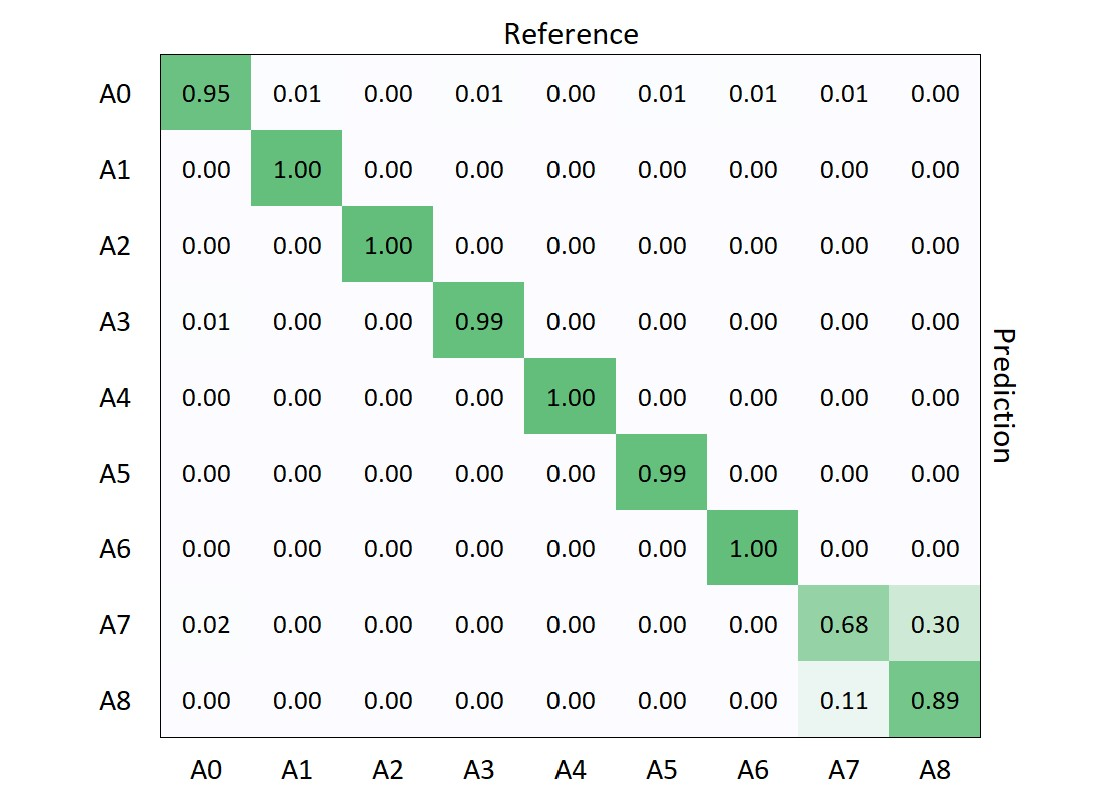
\includegraphics[width=7 cm]{Definitions/images/fnn_histogram_set.jpg}
	\caption{Normalized confusion matrix for FNN classifier using histogram dataset(set\_B). A0 in this table stands for non-exercise data points.}
	\label{fig:fnn_hbins_confusion_matrix}
\end{figure} 

\hosein{regarding We observe that when the standard activity recognition system is used with randomly oriented sensors (the random rotation case), the accuracy drops by 21.21\% on the average}
\subsubsection{RQ3: How are different evaluation methods?}
In this experiment, we asses the models by two (harder?) evaluation methods named Leave-One-Subject-Out cross validation and Leave-One-Trial-Out Cross validation. The goal here is to see how different ways of splitting data into train and test has impact on results. In K-fold since taking samples occurs on one unique dataset and each sample has overlap with two neighbour samples, there is always an overlap between train and test sets. therefore the model wasn't totally blind upon test set during training. Using LOTO and LOSO, we evaluate the model on a totally new dataset. Figure \ref{fig:evaluation_comparison} compares the performance of the models evaluating by 10-Fold, LOTO, and LOSO. For each classifier, results in the left columns have been obtained using 10-Fold evaluation, LOTO in the middle columns, and right columns are the results of LOSO cross validation. From the results, it is obvious that independent from featureset or classifier, evaluating by LOTO or LOSO gives a lower performance (~4\% and ~19\% respectively). This difference in results clearly shows that results of LOSO is also degraded due to performing differently an exercise by subjects. It is important to mention that this effect is surpassed in LOTO since subjects who have participated in training dataset, also participate in testing dataset. To compare classifiers, still FNN and SVM deliver the best result on all featuresets. The reason why we prefer to compare featuresets at first level is because they make more significant changes performance over different evaluation methods, as shown in Figure \ref{fig:evaluation_comparison}.
\begin{figure}[H]
	\centering
	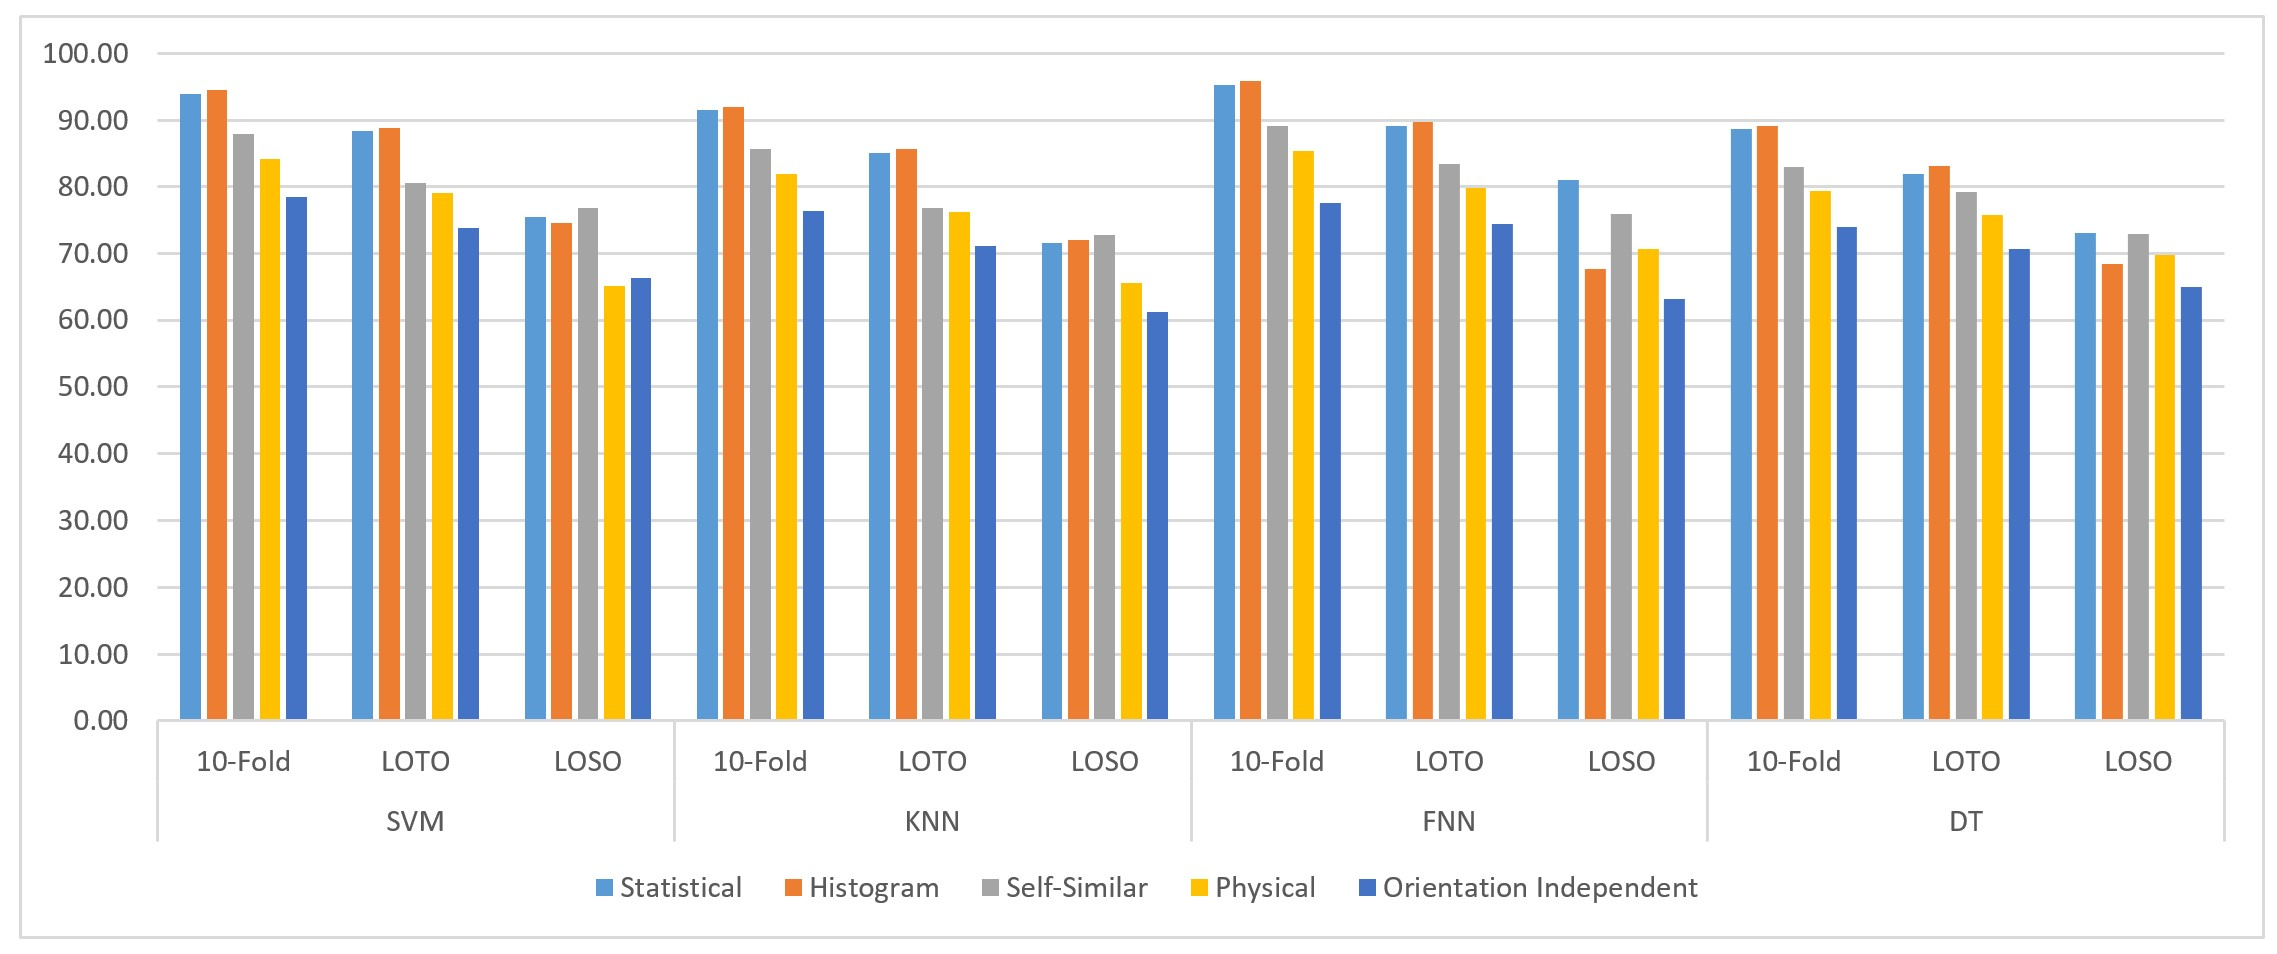
\includegraphics[width=14 cm]{Definitions/images/evaluation_comparison.jpg}
	\caption{Comparison between evaluation methods (10-Fold, LOTO, LOSO)}
	\label{fig:evaluation_comparison}
\end{figure} 

\begin{table}[H]
	\caption{Accuracy for each classifier and for all each feature-set using Leave-One-Trial-Out cross validation }
	\centering
	\begin{tabular}{p{3cm}p{2cm}p{2cm}p{2cm}p{2cm}p{2cm}}
		\toprule
		\textbf{Classifier} & \textbf{Set\_A} & \textbf{Set\_B} & \textbf{Set\_C} & \textbf{Set\_D} & \textbf{Set\_E} \\
		\midrule	
		SVM &  \cellcolor{gray!35}{76.73\%} & 73.11\% & \cellcolor{gray!35}{76.70}\% &69.19\% & 62.13\% \\
		KNN & 72.91\% & 75.58\% & 74.24\% &70.36\% & 61.74\% \\
		FNN & \cellcolor{gray!35}{77.07}\% & \cellcolor{gray!35}{79.87\%} &  \cellcolor{gray!35}{76.06\%} &\cellcolor{gray!35}{73.04\%} & 66.60\% \\
		DT & 69.48\% & 71.70\% & 72.58\% &71.18\% & 65.34\% \\
		\bottomrule
	\end{tabular}
	\label{Table:LOTO_results}
\end{table}

\begin{table}[H]
	\caption{Accuracy for each classifier and for all each feature-set using Leave-One-Subject-Out cross validation }
	\centering
	\begin{tabular}{p{3cm}p{2cm}p{2cm}p{2cm}p{2cm}p{2cm}}
		\toprule
		\textbf{Classifier} & \textbf{Set\_A} & \textbf{Set\_B} & \textbf{Set\_C} & \textbf{Set\_D} & \textbf{Set\_E} \\
		\midrule	
		SVM &  \cellcolor{gray!35}{68.83\%} & 69.11\% & \cellcolor{gray!35}{76.70}\% &69.19\% & 62.13\% \\
		KNN & 72.91\% & 75.58\% & 74.24\% &70.36\% & 61.74\% \\
		FNN & \cellcolor{gray!35}{77.07}\% & \cellcolor{gray!35}{79.87\%} & 76.06\% &\cellcolor{gray!35}{73.04\%} & 66.60\% \\
		DT & 69.48\% & 71.70\% &  \cellcolor{gray!35}{72.58\%} &71.18\% & 65.34\% \\
		\bottomrule
	\end{tabular}
	\label{Table:LOSO_results}
\end{table}
\section{Discussion}
\subsection{K-fold Evaluation result is biased?}
As we argued earlier, each process has a drawback that might cause a negative impact on the methods. For instance, SNOW can produce biased results and the FNOW generates few samples. To face these problems, we propose the Leave-One-Trial-Out (LOTO) sample generation process.
From the literature, the most popular method to evaluate a HAR model is K-fold cross-validation. In this method the data splits into k equal parts. The k-1 parts go for training and one part left for test. This process repeats for each k, separately. Main aim of this method is to keep the test and train part separate from each other and use all the samples in train and test. However, in case of using the conventional sliding window (with n\% overlap) for generating data-samples it is impossible for samples to be completely separated from each other. It is because of the overlap period which is common between each two windows in a sequence. In other words, as mentioned in \cite{jordao2018human}, the result is always biased because n\% of the data are identical between test and train part. To avoid this drawback, a ordinary evaluation method is Leave-One-Subject-Out (LOSO). Basically, this method resembles the k-fold cross-validation in which a fold is replaced by a subject. This method is secure against being biased since the data from each subject has no common area with other subjects. However, in order to have the performance in a satisfactory level, we have to increase the number of subjects, respectively. The Leave-One-Trial-Out (LOTO) cross-validation\cite{jordao2018human} is similar to LOSO, but use the data of a trial instead of a subject. Thus, we have ensured that the samples are basically separated and the performance does not depend on the number of subjects any more.
\hosein{+ showing it in a example}

\subsection{Hand-Crafted Features VS Automated Features}

 Automatic feature learning

The extraction of hand-crafted features depends on domain knowledge. However, automatically learned features by the deep networks  features are
easy to understand and implement

The key advantage of using hand-crafted features is that the features are computationally lightweight to implement especially in ubiquitous devices (Morales et al., 2017).
The strengths of the automatically learned features by the deep networks are that the learning can be very deep, and the learning process does not rely on domain knowledge.


Feature type Advantages
Hand-crafted Features
Automatically learned features
Table 5 Comparison of hand-crafted features and automatically learned features Disadvantages
Easy to understand the physical meanings of the features; Extraction is efficient and easy to deploy; Work well for many HAR problems.
No domain knowledge needed; Automatically learning features from raw data; Features are more robust and generalized.
Domain knowledge needed; Sensor-type specific; Need further feature selection.
Lots of computing resources; Parameters are difficult to adjust; The learned features are less interpretable


Authors should discuss the results and how they can be interpreted in perspective of previous studies and of the working hypotheses. The findings and their implications should be discussed in the broadest context possible. Future research directions may also be highlighted.

Another way of evaluating the featuresets is using a feature selection method and compare the percentage of contribution of each featureset within the featureset result.


Using neural network in pattern recognition is one of the most promising topic in recent works, especially in activity recognition. It is because, the characteristics like flexibility of the model with more various activity sets or improving the performance by adding more data in training phase make NN an appealing choice to data analyst. Related works have presented successful approaches on customizing neural nets to solve certain problems in HAR. In most studies, the authors introduced a new design of layers and sort of new configuration of neurons in each layer. Their results show that NN works better rather traditional models like GLM or SVM on more complex activities, in practice.
\subsection{Learning Speed }
Histogram bins progress outperforms all other featuresets in delivering better accuracy in less training time.
\begin{figure}[H]
	\centering
	\begin{subfigure}{.5\textwidth}
		\centering
		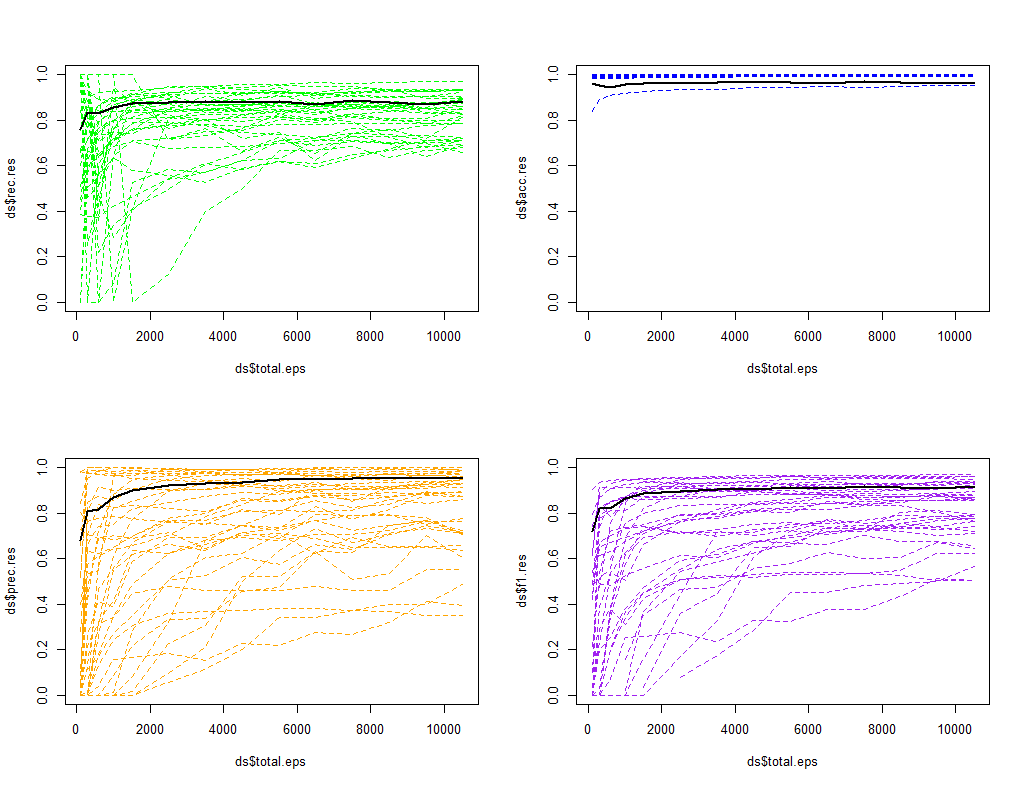
\includegraphics[width=1\linewidth]{Definitions/images/fnn_statistical_set.png}
		\caption{Statistical features}
		\label{fig:fnn_balanced}
	\end{subfigure}%
	\begin{subfigure}{.5\textwidth}
		\centering
		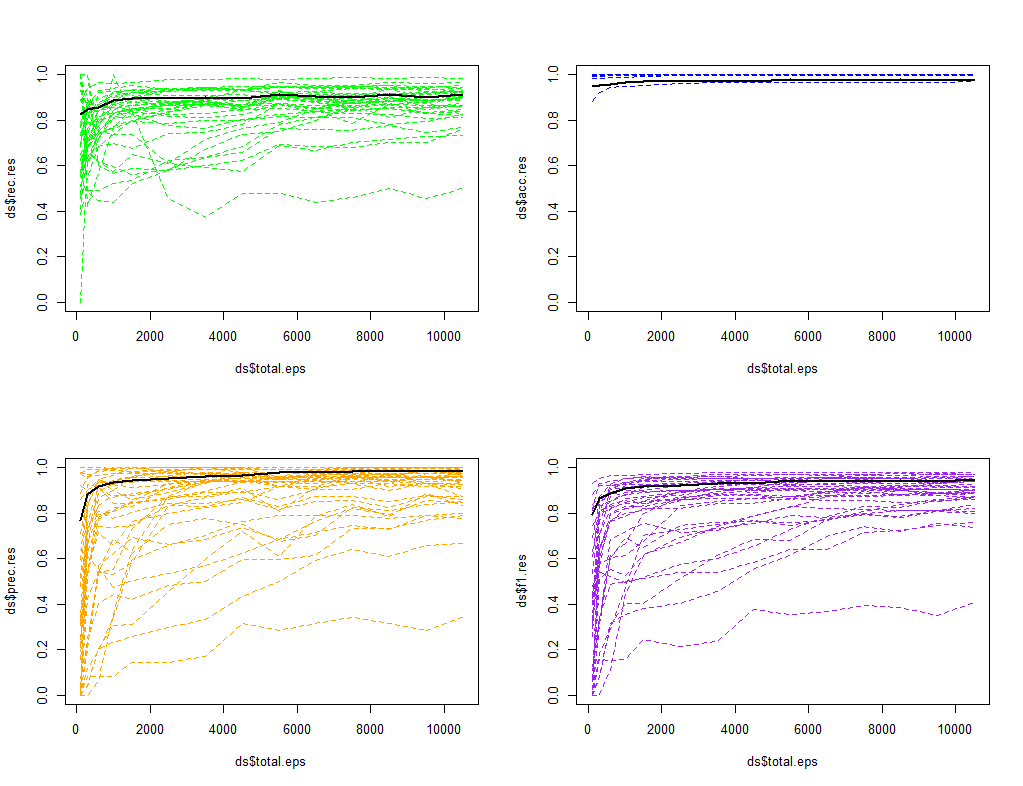
\includegraphics[width=1\linewidth]{Definitions/images/fnn_hbin_set.png}
		\caption{Histogram features}
		\label{fig:fnn_imbalanced}
	\end{subfigure}%
	\caption{Comparing impact of featureset on FNN convergence speed}
	\label{fig:imbalance_dataset}
\end{figure} 


%%%%%%%%%%%%%%%%%%%%%%%%%%%%%%%%%%%%%%%%%%
\section{Conclusions}
In this paper, a human activity recognition framework
based on feature selection techniques is presented. We examined three feature selection methods and found that the sequential forward selection (SFS) method achieved the best performance compared to Relief-F and single feature classification (SFC) methods. In addition, we have demonstrated that our self-designed physical features make significant contributions to the recognition system. Finally, we have shown that the feature selection framework with a hierarchical structure improves the recognition performance compared to the single-layer framework. However, the structure of the hierarchical framework, i.e. how the different classes are arranged in meta-classes, is designed manually, based on domain knowledge. Although this type of knowledge may generally be helpful when designing recognition systems, in our future work, we will explore methods to learn the structure automatically in a data-driven manner.
%%%%%%%%%%%%%%%%%%%%%%%%%%%%%%%%%%%%%%%%%%
\vspace{6pt} 

%%%%%%%%%%%%%%%%%%%%%%%%%%%%%%%%%%%%%%%%%%
%% optional
%\supplementary{The following are available online at \linksupplementary{s1}, Figure S1: title, Table S1: title, Video S1: title.}

% Only for the journal Methods and Protocols:
% If you wish to submit a video article, please do so with any other supplementary material.
% \supplementary{The following are available at \linksupplementary{s1}, Figure S1: title, Table S1: title, Video S1: title. A supporting video article is available at doi: link.}

%%%%%%%%%%%%%%%%%%%%%%%%%%%%%%%%%%%%%%%%%%
\authorcontributions{For research articles with several authors, a short paragraph specifying their individual contributions must be provided. The following statements should be used ``conceptualization, X.X. and Y.Y.; methodology, X.X.; software, X.X.; validation, X.X., Y.Y. and Z.Z.; formal analysis, X.X.; investigation, X.X.; resources, X.X.; data curation, X.X.; writing--original draft preparation, X.X.; writing--review and editing, X.X.; visualization, X.X.; supervision, X.X.; project administration, X.X.; funding acquisition, Y.Y.'', please turn to the  \href{http://img.mdpi.org/data/contributor-role-instruction.pdf}{CRediT taxonomy} for the term explanation. Authorship must be limited to those who have contributed substantially to the work reported.}

%%%%%%%%%%%%%%%%%%%%%%%%%%%%%%%%%%%%%%%%%%
\funding{Please add: ``This research received no external funding'' or ``This research was funded by NAME OF FUNDER grant number XXX.'' and  and ``The APC was funded by XXX''. Check carefully that the details given are accurate and use the standard spelling of funding agency names at \url{https://search.crossref.org/funding}, any errors may affect your future funding.}

%%%%%%%%%%%%%%%%%%%%%%%%%%%%%%%%%%%%%%%%%%
\acknowledgments{In this section you can acknowledge any support given which is not covered by the author contribution or funding sections. This may include administrative and technical support, or donations in kind (e.g., materials used for experiments).}

%%%%%%%%%%%%%%%%%%%%%%%%%%%%%%%%%%%%%%%%%%
\conflictsofinterest{Declare conflicts of interest or state ``The authors declare no conflict of interest.'' Authors must identify and declare any personal circumstances or interest that may be perceived as inappropriately influencing the representation or interpretation of reported research results. Any role of the funders in the design of the study; in the collection, analyses or interpretation of data; in the writing of the manuscript, or in the decision to publish the results must be declared in this section. If there is no role, please state ``The funders had no role in the design of the study; in the collection, analyses, or interpretation of data; in the writing of the manuscript, or in the decision to publish the results''.} 

%%%%%%%%%%%%%%%%%%%%%%%%%%%%%%%%%%%%%%%%%%
%% optional
\abbreviations{The following abbreviations are used in this manuscript:\\
	
	\noindent 
	\begin{tabular}{@{}ll}
		MDPI & Multidisciplinary Digital Publishing Institute\\
		DOAJ & Directory of open access journals\\
		TLA & Three letter acronym\\
		LD & linear dichroism
\end{tabular}}

%%%%%%%%%%%%%%%%%%%%%%%%%%%%%%%%%%%%%%%%%%
%% optional
\appendixtitles{no} %Leave argument "no" if all appendix headings stay EMPTY (then no dot is printed after "Appendix A"). If the appendix sections contain a heading then change the argument to "yes".
\appendix
\section{}
\unskip
\subsection{}
The appendix is an optional section that can contain details and data supplemental to the main text. For example, explanations of experimental details that would disrupt the flow of the main text, but nonetheless remain crucial to understanding and reproducing the research shown; figures of replicates for experiments of which representative data is shown in the main text can be added here if brief, or as Supplementary data. Mathematical proofs of results not central to the paper can be added as an appendix.

\section{}
All appendix sections must be cited in the main text. In the appendixes, Figures, Tables, etc. should be labeled starting with `A', e.g., Figure A1, Figure A2, etc. 

%%%%%%%%%%%%%%%%%%%%%%%%%%%%%%%%%%%%%%%%%%
% Citations and References in Supplementary files are permitted provided that they also appear in the reference list here. 

%=====================================
% References, variant A: internal bibliography
%=====================================
\reftitle{References}
%\begin{thebibliography}{999}
%	% Reference 1
%	\bibitem[Author1(year)]{ref-journal}
%	Author1, T. The title of the cited article. {\em Journal Abbreviation} {\bf 2008}, {\em 10}, 142--149.
%	% Reference 2
%	\bibitem[Author2(year)]{ref-book}
%	Author2, L. The title of the cited contribution. In {\em The Book Title}; Editor1, F., Editor2, A., Eds.; Publishing House: City, Country, 2007; pp. 32--58.
%\end{thebibliography}

% The following MDPI journals use author-date citation: Arts, Econometrics, Economies, Genealogy, Humanities, IJFS, JRFM, Laws, Religions, Risks, Social Sciences. For those journals, please follow the formatting guidelines on http://www.mdpi.com/authors/references
% To cite two works by the same author: \citeauthor{ref-journal-1a} (\citeyear{ref-journal-1a}, \citeyear{ref-journal-1b}). This produces: Whittaker (1967, 1975)
% To cite two works by the same author with specific pages: \citeauthor{ref-journal-3a} (\citeyear{ref-journal-3a}, p. 328; \citeyear{ref-journal-3b}, p.475). This produces: Wong (1999, p. 328; 2000, p. 475)

%=====================================
% References, variant B: external bibliography
%=====================================
\externalbibliography{yes}
\bibliography{mybib}

%%%%%%%%%%%%%%%%%%%%%%%%%%%%%%%%%%%%%%%%%%
%% optional
\sampleavailability{Samples of the compounds ...... are available from the authors.}

%% for journal Sci
%\reviewreports{\\
%Reviewer 1 comments and authors’ response\\
%Reviewer 2 comments and authors’ response\\
%Reviewer 3 comments and authors’ response
%}

%%%%%%%%%%%%%%%%%%%%%%%%%%%%%%%%%%%%%%%%%%
\end{document}
